\chapter{Recunoașterea alfabetului ASL}
\label{cap:cap2}

\section{Construirea setului de date}

\textbf{Extragerea cadrelor din videoclipuri}. În cazul seturilor de date formate din clipuri video, a fost utilizat un script \textbf{Python} \cite{python312}, care extrage și salvează cadrele citite cu ajutorul bibliotecii \textbf{OpenCV} \cite{opencv_library}, utilă în procesarea și analiza imaginilor.

\textbf{Extragerea palmei din imagini}. Pentru a extrage mâna, a fost utilizat algoritmul \textbf{MediaPipe Hands}, dezvoltat de \textbf{Google} \cite{zhang2020mediapipehandsondevicerealtime} pentru detecția palmei într-o imagine. Acest pas a fost necesar pentru a elimina zgomotul creat de fundal sau de fețele oamenilor și pentru a aduce palma în prim plan. Transformarea unei imagini în urma aplicării algoritmului poate fi observată în Figura~\ref{fig:before_after_mediapipe}.

În cazul cadrelor extrase din videoclipuri și al palmelor extrase din imagini, imaginile invalide (neclaritate, poziție greșită a mâinii, mână incorectă etc.) au fost eliminate manual.

\begin{figure}[H]
  \centering
  \begin{subfigure}{0.3\textwidth}
  \centering
    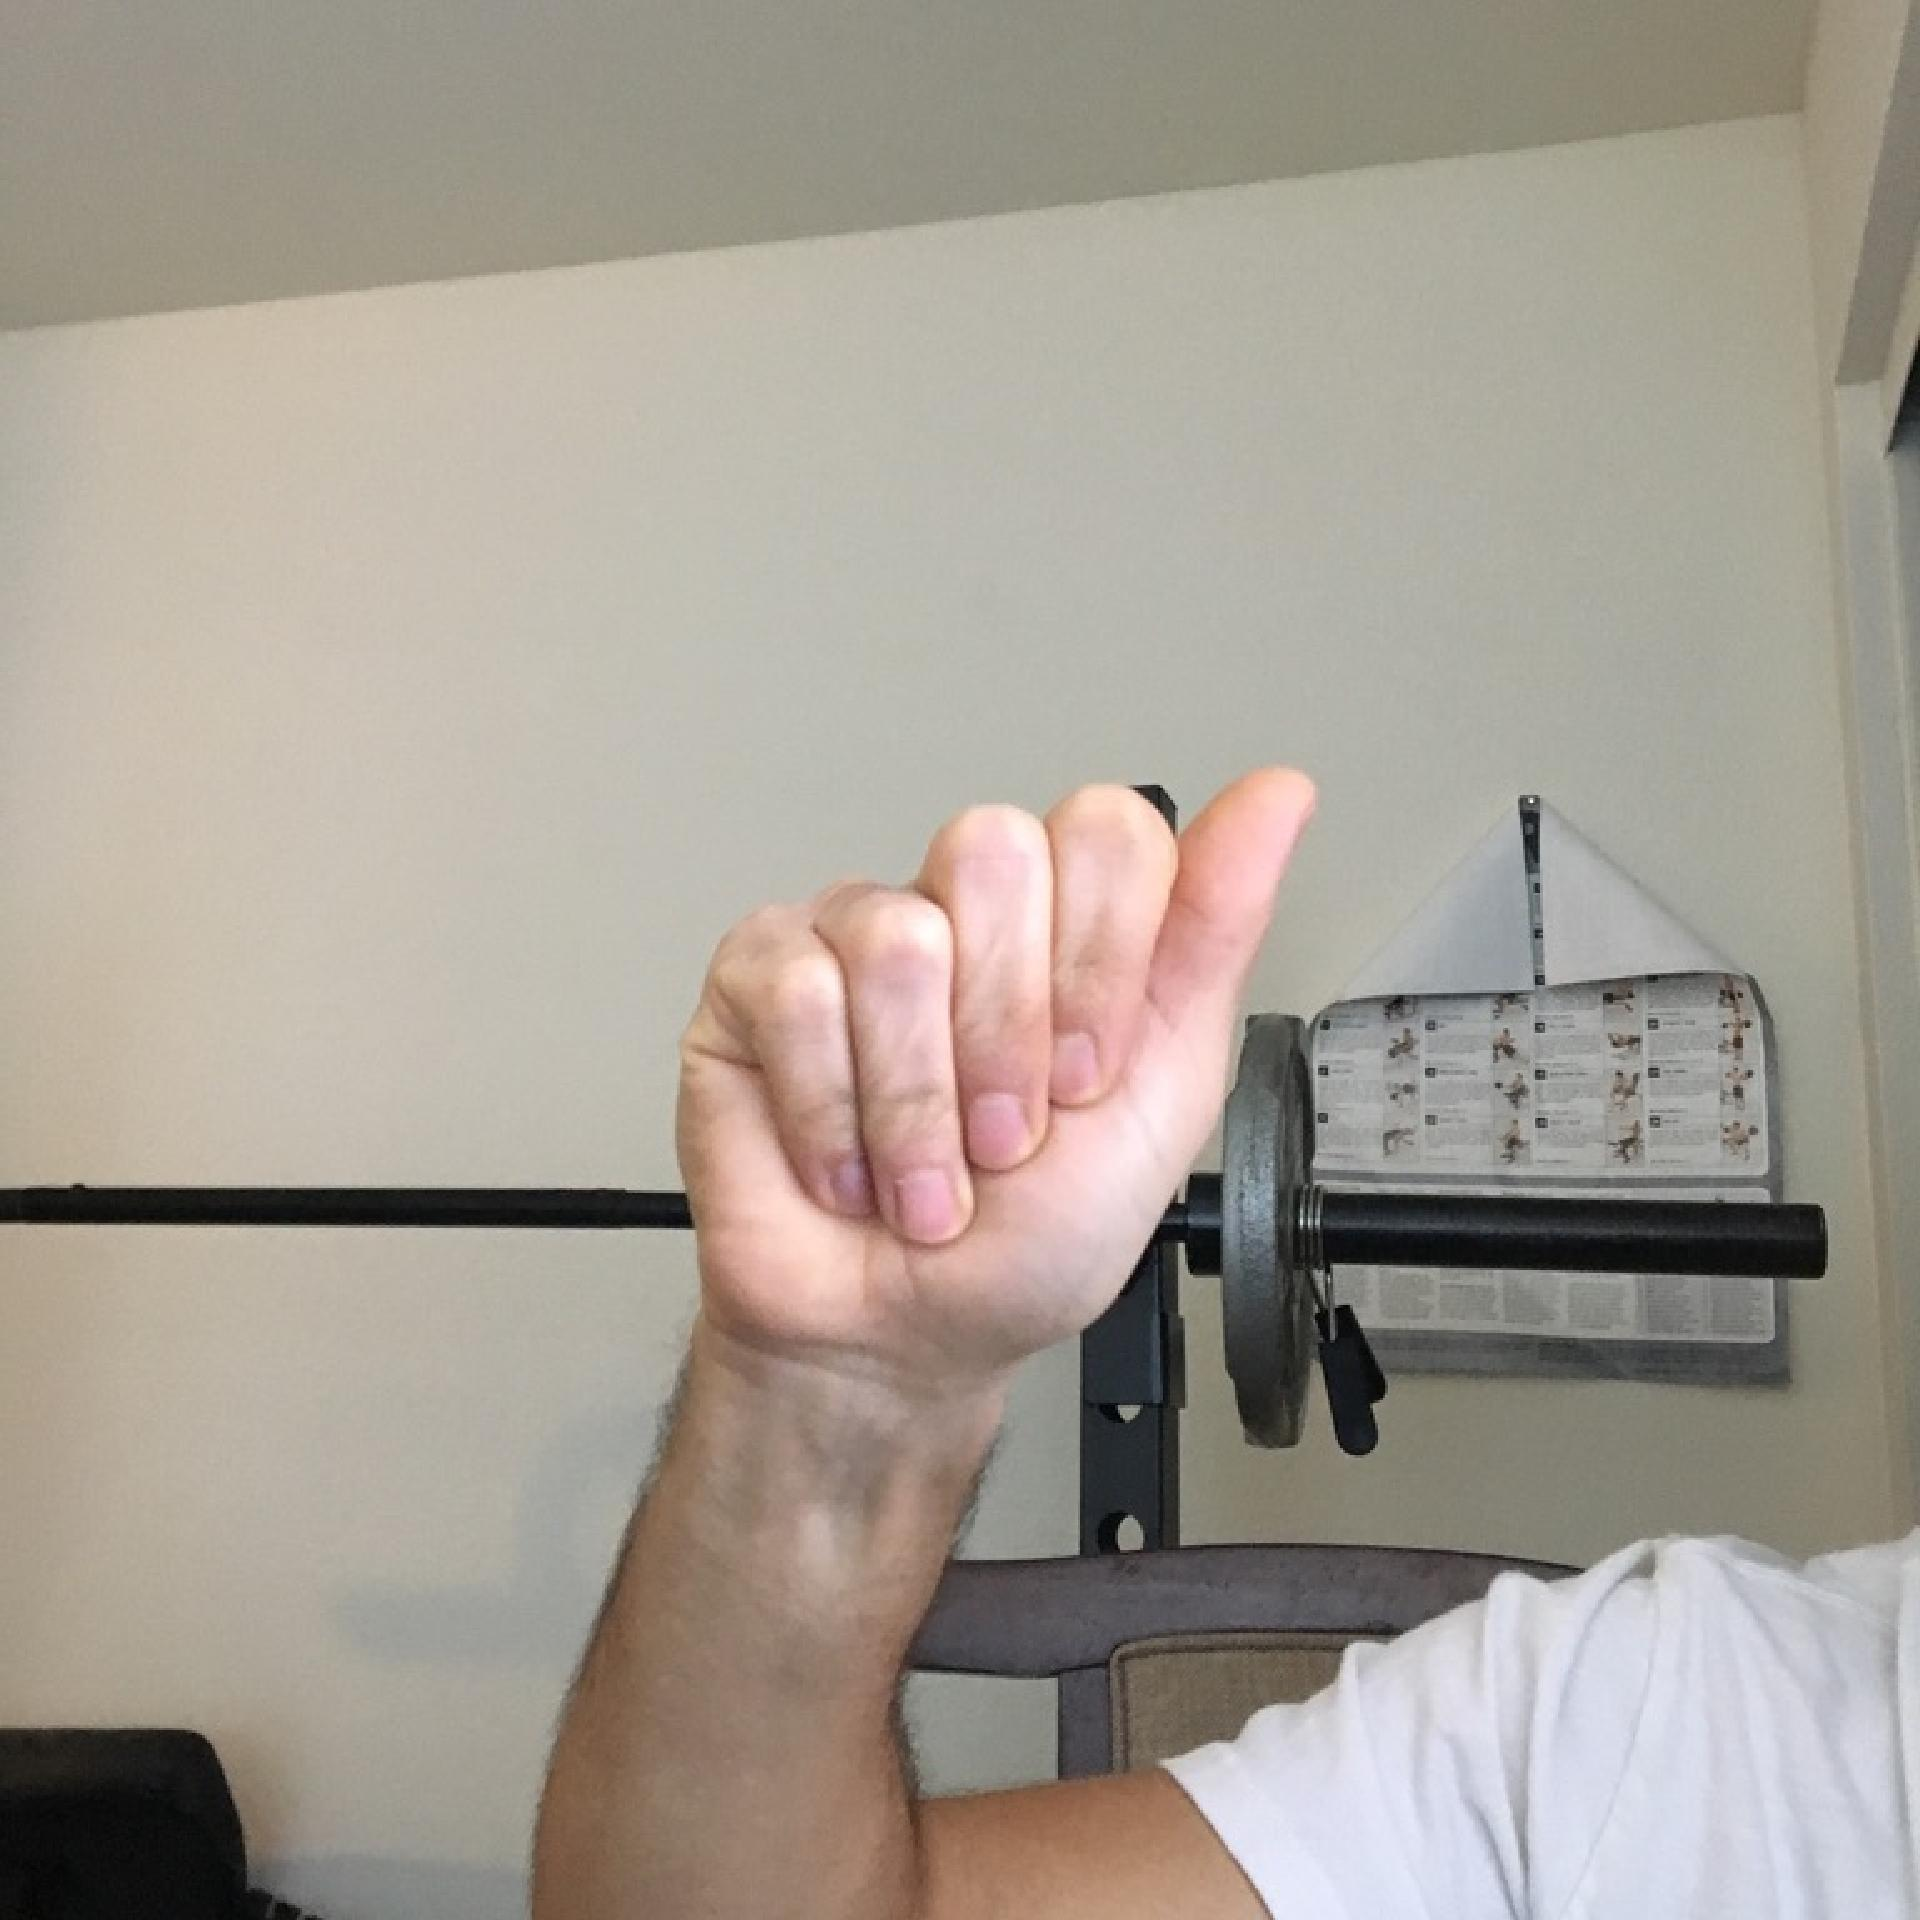
\includegraphics[width=4cm,height=4cm,keepaspectratio]
{images/2-recunoasterea-asl/exemple_litera_a/a_before_mediapipe.jpg}
    \caption{}
  \end{subfigure}
  \hspace{0.1\textwidth}
  \begin{subfigure}{0.3\textwidth}
    \centering
    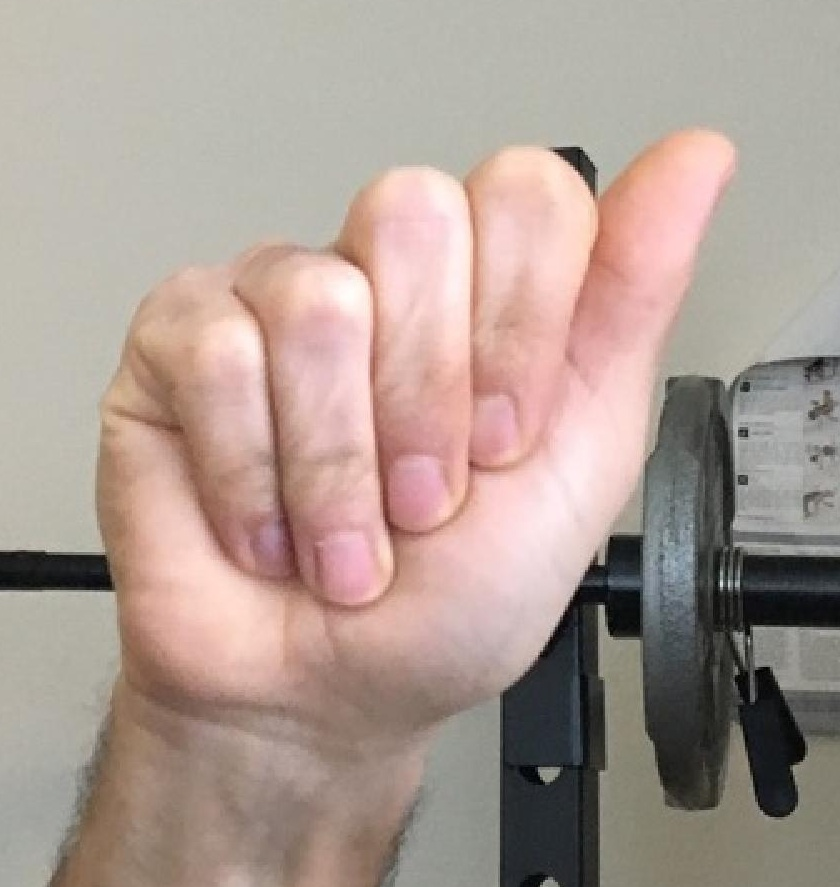
\includegraphics[width=4cm,height=4cm,keepaspectratio]
{images/2-recunoasterea-asl/exemple_litera_a/a_after_mediapipe.jpg}
    \caption{}
  \end{subfigure}
  \caption[Aplicarea MediaPipe Hands]{\textbf{Aplicarea MediaPipe Hands}. \textit{(a) prezintă imaginea originală care servește drept intrare pentru MediaPipe Hands; (b) este imaginea utilizată în antrenare, în urma extragerii acesteia. Se poate observa cum palma devine obiectul principal al imaginii.}}
  \label{fig:before_after_mediapipe}
\end{figure}

\textbf{Împărțirea setului de date}.
Pentru a ne asigura că acuratețea obținută pe seturile de validare și testare reflectă performanța în lumea reală, imaginile sunt împărțite manual, în funcție de sursa lor, astfel încât în seturile de validare și testare să nu existe imagini cu mâini sau fundaluri aflate în setul de de antrenare. În final, avem un total de 36.871 de imagini, împărțite după cum urmează: pentru setul de antrenare sunt alocate 30.450 de imagini, reprezentând 82,58\% din total, pentru setul de validare 3.211 de imagini, reprezentând 8,7\% din total, iar pentru setul de testare 3.210 de imagini, reprezentând 8,7\% din total.

\textbf{Distribuția claselor}. În cazul setului de antrenare, literele subreprezentate sunt M, N și P. Cauza acestei subreprezentări este dificultatea pe care am întâlnit-o în colectarea unui număr suficient de exemple pentru un singur dialect. Cu toate acestea, un număr de aproximativ 1.000 de exemple pentru o clasă este considerat a fi suficient pentru ca modelul să poată învăța trăsăturile importante.

În cazul seturilor de validare și testare, distribuția este aproximativ egală, deoarece clasele nu au necesitat un număr ridicat de exemple, spre deosebire de cele care formează setul de antrenare. Distribuția exactă a seturilor poate fi observată în Figura~\ref{fig:class_distrib}.

\begin{figure}[H]
  \centering
  \begin{subfigure}{0.49\textwidth}
    \centering
    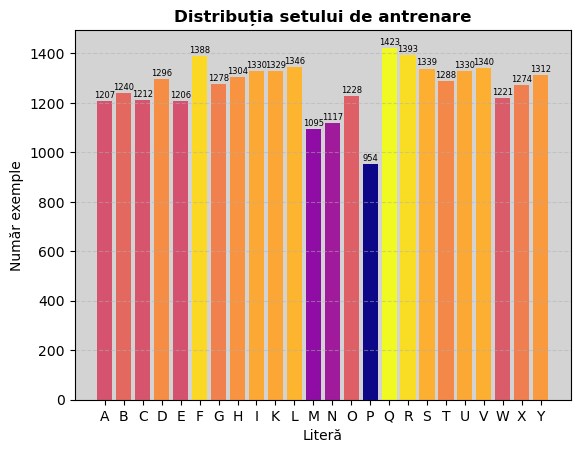
\includegraphics[width=\linewidth]{images/2-recunoasterea-asl/train_classes_distrib.png}
    \caption{}
  \end{subfigure}
  \begin{subfigure}{0.49\textwidth}
    \centering
    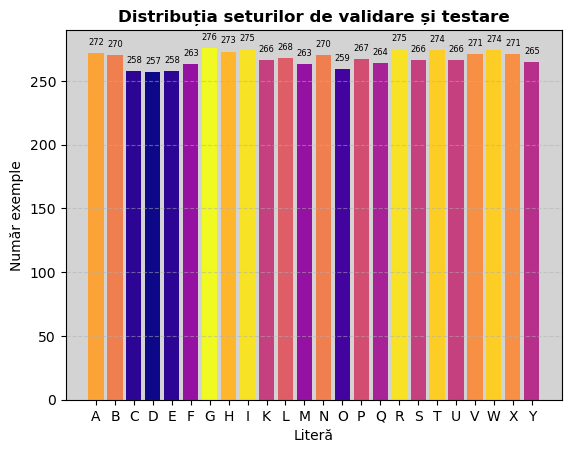
\includegraphics[width=\linewidth]{images/2-recunoasterea-asl/test_val_classes_distrib.png}
    \caption{}
  \end{subfigure}
  \caption[Distribuția claselor]{\textbf{Distribuția claselor}. \textit{(a) ilustrează distribuția setului de antrenare; (b) ilustrează distribuția setului care este împărțit aleator ($seed = 42$), în două seturi: validare și testare.}}
  \label{fig:class_distrib}
\end{figure}

\section{Preprocesarea imaginilor}

\textbf{Preprocesarea setului de antrenare}. Cu scopul de a avea exemple cât mai variate, în special pentru a combate probleme ca \textit{overfitting}-ul, am decis să utilizăm o tehnică numită augmentarea datelor. Efectele clasice (intra-imagine), care acționează independent asupra unei singure imagini, precum răsturnarea, rotirea, aplicarea de estompare sau zgomot, modificarea culorilor sau ștergerea unei porțiuni dintr-o imagine, pot îmbunătăți capacitatea de generalizare a unui model deep, cum ar fi un CNN \cite{data_augment1, data_augment2}. Pe lângă efectele intra-imagine, există și efecte care amestecă două imagini, efecte inter-imagine, cum ar fi \textit{CutMix} \cite{cutmix} și \textit{MixUp} \cite{mixup}.

Pentru efectele clasice, augmentările au fost realizate utilizând biblioteca \textbf{Albumentations} \cite{albumentations}. Augmentările aplicate sunt: răsturnare orizontală cu probabilitatea aplicării de 50\%, rotire între $-15^\circ$ și $15^\circ$ cu o probabilitate de 40\%, estompare cu filtru de dimensiune 3x3 și probabilitate de 30\%, zgomot Gaussian cu abatere standard între 0.05 și 0.07 și o probabilitate de 30\% și trepidație de culoare sau \textit{color jitter} (schimbarea luminozității, contrastului, saturației și nuanței), cu o probabilitate de 40\%. Toate imaginile sunt redimensionate la $224 \times 224$, normalizate folosind media per canal RGB $[0.5797, 0.5104, 0.4846]$ și abatere standard $[0.1804, 0.1845, 0.1883]$, reprezentând media și abaterea standard a setului de antrenare, și în final, transformate în tensori. 

După cum se observă în Figura~\ref{fig:exemplu_efecte_clasice}, efectele aplicate pot ajuta modelul să „înțeleagă” că factori precum culoarea pielii sau poziția exactă a mâinii nu sunt importanți, și mai mult de atât, să se descurce în condiții de luminozitate scăzută și cu imagini de calitate redusă.
 
\begin{figure}[H]
  \centering
 \begin{subfigure}{0.18\textwidth}
      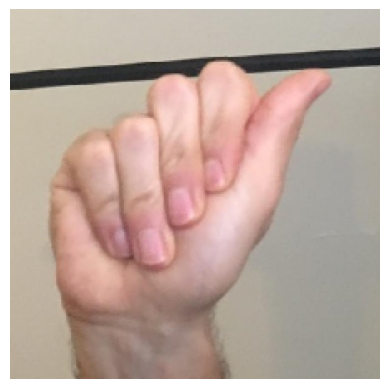
\includegraphics[width=\linewidth]{images/2-recunoasterea-asl/imagine_a_originala.png}
      \caption{}
    \end{subfigure}
    \begin{subfigure}{0.18\textwidth}
      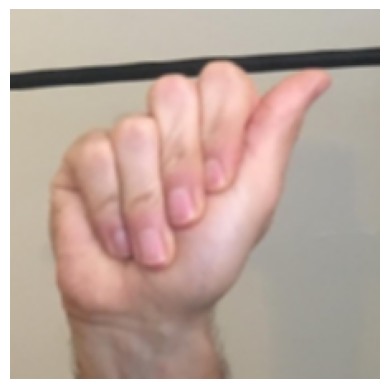
\includegraphics[width=\linewidth]{images/2-recunoasterea-asl/imagine_a_blur.png}
      \caption{}
    \end{subfigure}
    \hspace{0.005\textwidth}
    \begin{subfigure}{0.18\textwidth}
      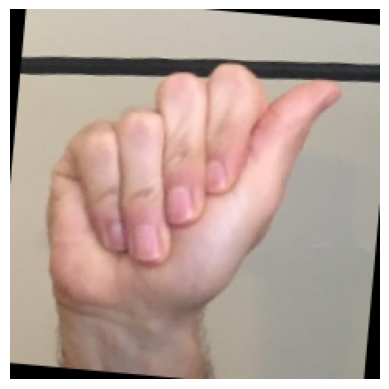
\includegraphics[width=\linewidth]{images/2-recunoasterea-asl/imagine_a_rotate.png}
      \caption{}
    \end{subfigure}
    \hspace{0.005\textwidth}
    \begin{subfigure}{0.18\textwidth}
      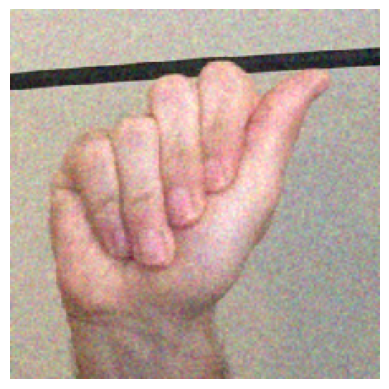
\includegraphics[width=\linewidth]{images/2-recunoasterea-asl/imagine_a_gauss_noise.png}
      \caption{}
    \end{subfigure}
    \hspace{0.005\textwidth}
    \begin{subfigure}{0.18\textwidth}
      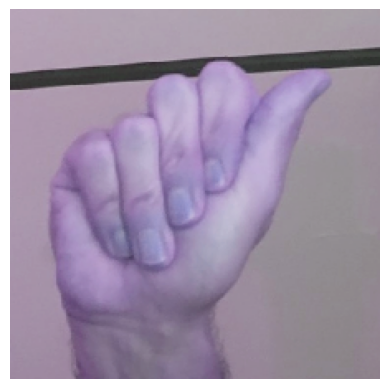
\includegraphics[width=\linewidth]{images/2-recunoasterea-asl/imagine_a_color_jitter.png}
      \caption{}
    \end{subfigure}

  \caption[Efecte intra-imagine]{\textbf{Efecte intra-imagine}. \textit{Ilustrăm efectele aplicate asupra imaginilor, pentru augmentarea setului de antrenare. (a) exemplifică imaginea originală, (b) exemplifică efectul de estompare, (c) exemplifică rotirea, (d) exemplifică zgomotul adăugat, iar (e) exemplifică efectul de color jitter.}}
  \label{fig:exemplu_efecte_clasice}
\end{figure}

În cazul efectelor inter-imagine CutMix și MixUp am utilizat biblioteca \textbf{torchvision} \cite{torchvision2016}. La fiecare încărcare a unui \textit{batch} de date din setul de antrenare, cu ajutorul unui obiect de tip \textit{DataLoader} din biblioteca \textbf{PyTorch} \cite{pytorch}, alegem aleatoriu dintre CutMix sau MixUp, cu o probabilitate de aplicare de 50\%. 

CutMix este definit ca:
\begin{equation}
    \begin{aligned}
        \tilde{x} &= M \odot x_B + (1 - M) \odot x_A \\
        \tilde{y} &= \lambda y_A + (1 - \lambda) y_B
    \end{aligned}
    \label{eq:cutmix}
\end{equation}
unde $\tilde{x}$ este imaginea rezultată, $x_B$ și $x_A$ sunt imaginile sursă care vor fi combinate, iar $M$ este masca binară care va fi înmulțită element cu element ($\odot$) cu imaginile sursă. $\tilde{y}$ este eticheta \textit{soft}, iar $\lambda$ reprezintă ponderea fiecărei imagini în imaginea finală.

MixUp este definit ca:
\begin{equation}
    \begin{aligned}
        \tilde{x} &= \lambda x_A + (1 - \lambda) x_B \\
        \tilde{y} &= \lambda y_A + (1 - \lambda) y_B
    \end{aligned}
    \label{eq:cutmix}
\end{equation}
unde $\tilde{x}$ este imaginea rezultată, $x_A$ și $x_B$ sunt imaginile sursă care vor fi combinate, iar $\lambda$ este un coeficient ales aleator, care controlează proporția fiecărei imagini. $\tilde{y}$ este la fel ca și în cazul ecuației pentru CutMix.

Este important de menționat că, în cazul nostru, păstrăm din tehnica CutMix și MixUp doar combinarea imaginilor, iar eticheta atribuită corespunde clasei dominante din imaginea compusă.

Pentru a vizualiza efectele aplicate asupra a două imagini, vezi Figura~\ref{fig:exemplu_efecte_avansate}.

\begin{figure}[H]
  \centering
    \begin{subfigure}{0.22\textwidth}
      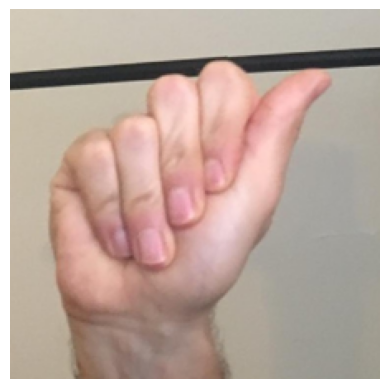
\includegraphics[width=\linewidth]{images/2-recunoasterea-asl/ctmx_mxup_orig_1.png}
      \caption{}
    \end{subfigure}
    \hspace{0.001\textwidth}
    \begin{subfigure}{0.22\textwidth}
      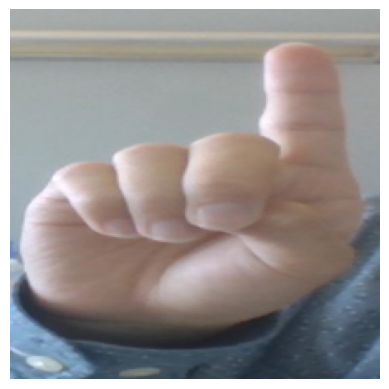
\includegraphics[width=\linewidth]{images/2-recunoasterea-asl/ctmx_mxup_orig_2.png}
      \caption{}
    \end{subfigure}
    \hspace{0.001\textwidth}
    \begin{subfigure}{0.25\textwidth}
      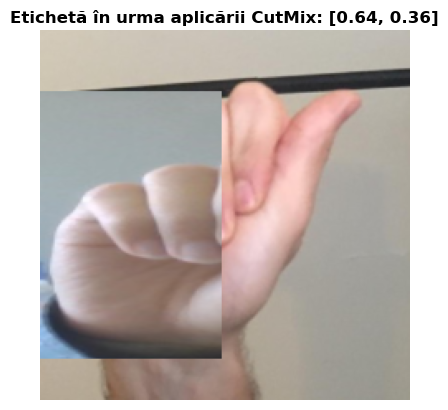
\includegraphics[width=\linewidth]{images/2-recunoasterea-asl/ctmx_img_1.png}
      \caption{}
    \end{subfigure}
    \hspace{0.001\textwidth}
    \begin{subfigure}{0.25\textwidth}
      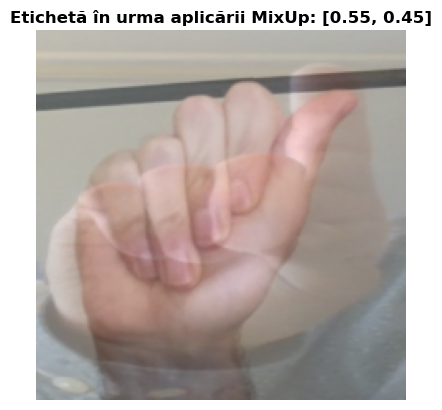
\includegraphics[width=\linewidth]{images/2-recunoasterea-asl/mxup_img_1.png}
      \caption{}
    \end{subfigure}

  \caption[CutMix și MixUp]{\textbf{CutMix și MixUp}. \textit{Ilustrăm efectele CutMix și MixUp. (a) și (b) reprezintă două exemple din două clase distincte; (c) exemplifică efectul CutMix, unde clasa din (a) are o pondere de 0.64, iar (b) are o pondere de 0.36; (d) exemplifică efectul MixUp, unde clasa (a) are o pondere de 0.55, iar clasa (b) are o pondere de 0.45.}}
  \label{fig:exemplu_efecte_avansate}
\end{figure}

\textbf{Preprocesarea seturilor de validare și testare}. În cazul acestor două seturi, imaginea originală este redimensionată 
la $224 \times 224$, normalizată cu media și abaterea standard a setului de antrenare și transformată în tensori.

\section{Arhitectura modelului}

Arhitectura creată pentru acest studiu a fost inspirată din mai multe arhitecturi revoluționare, precum VGG \cite{vggnet} de unde a fost preluată ideea utilizării de bloc (mai multe straturi) convoluțional, urmat de un strat de \textit{max pooling}, tehnică care reduce dimensiunea hărților de activare.

În plus, arhitecura a fost inspirată de ResNet \cite{resnet}, prin inserarea unor straturi convoluționale succesive care păstrează numărul de canale, consolidând și rafinând trăsăturile extrase în ultima extindere. Din aceeași arhitectură, a fost inspirată și inserarea straturilor de \textit{batch normalization} după straturile convoluționale, cu scopul de a accelerara procesul de învățare, permițând utilizarea unei rate de învățare mai mare, și de a oferi o ușoară regularizare prin reducerea variațiilor
mari \cite{batch_norm}. În final, a fost preluată și tehnica de \textit{adaptive average pooling}, prin care este redusă înălțimea și lățimea imaginii la $1\times1$, păstrând adâncimea (numărul canalelor).

Modelul este format din 12 straturi convoluționale, fiecare urmat de câte un strat de batch normalization și activat cu ajutorul funcției de activare ReLU, fiind una dintre cele mai utilizate funcții de activare în cazul modelelor de tip CNN, deoarece oferă acuratețe ridicată în sarcini precum clasificarea imaginilor \cite{relu1, relu2}. În final, este prezent un clasificator format din două straturi complet conectate (dense). Straturile convoluționale sunt împărțite în cinci blocuri care sunt explicate în continuare. Pentru o mai bună înțelegere a arhitecturii și a explicației ce urmează, vezi Figura~\ref{fig:diagrama_vladimirnet}.

\begin{figure}[H]
  \centering
  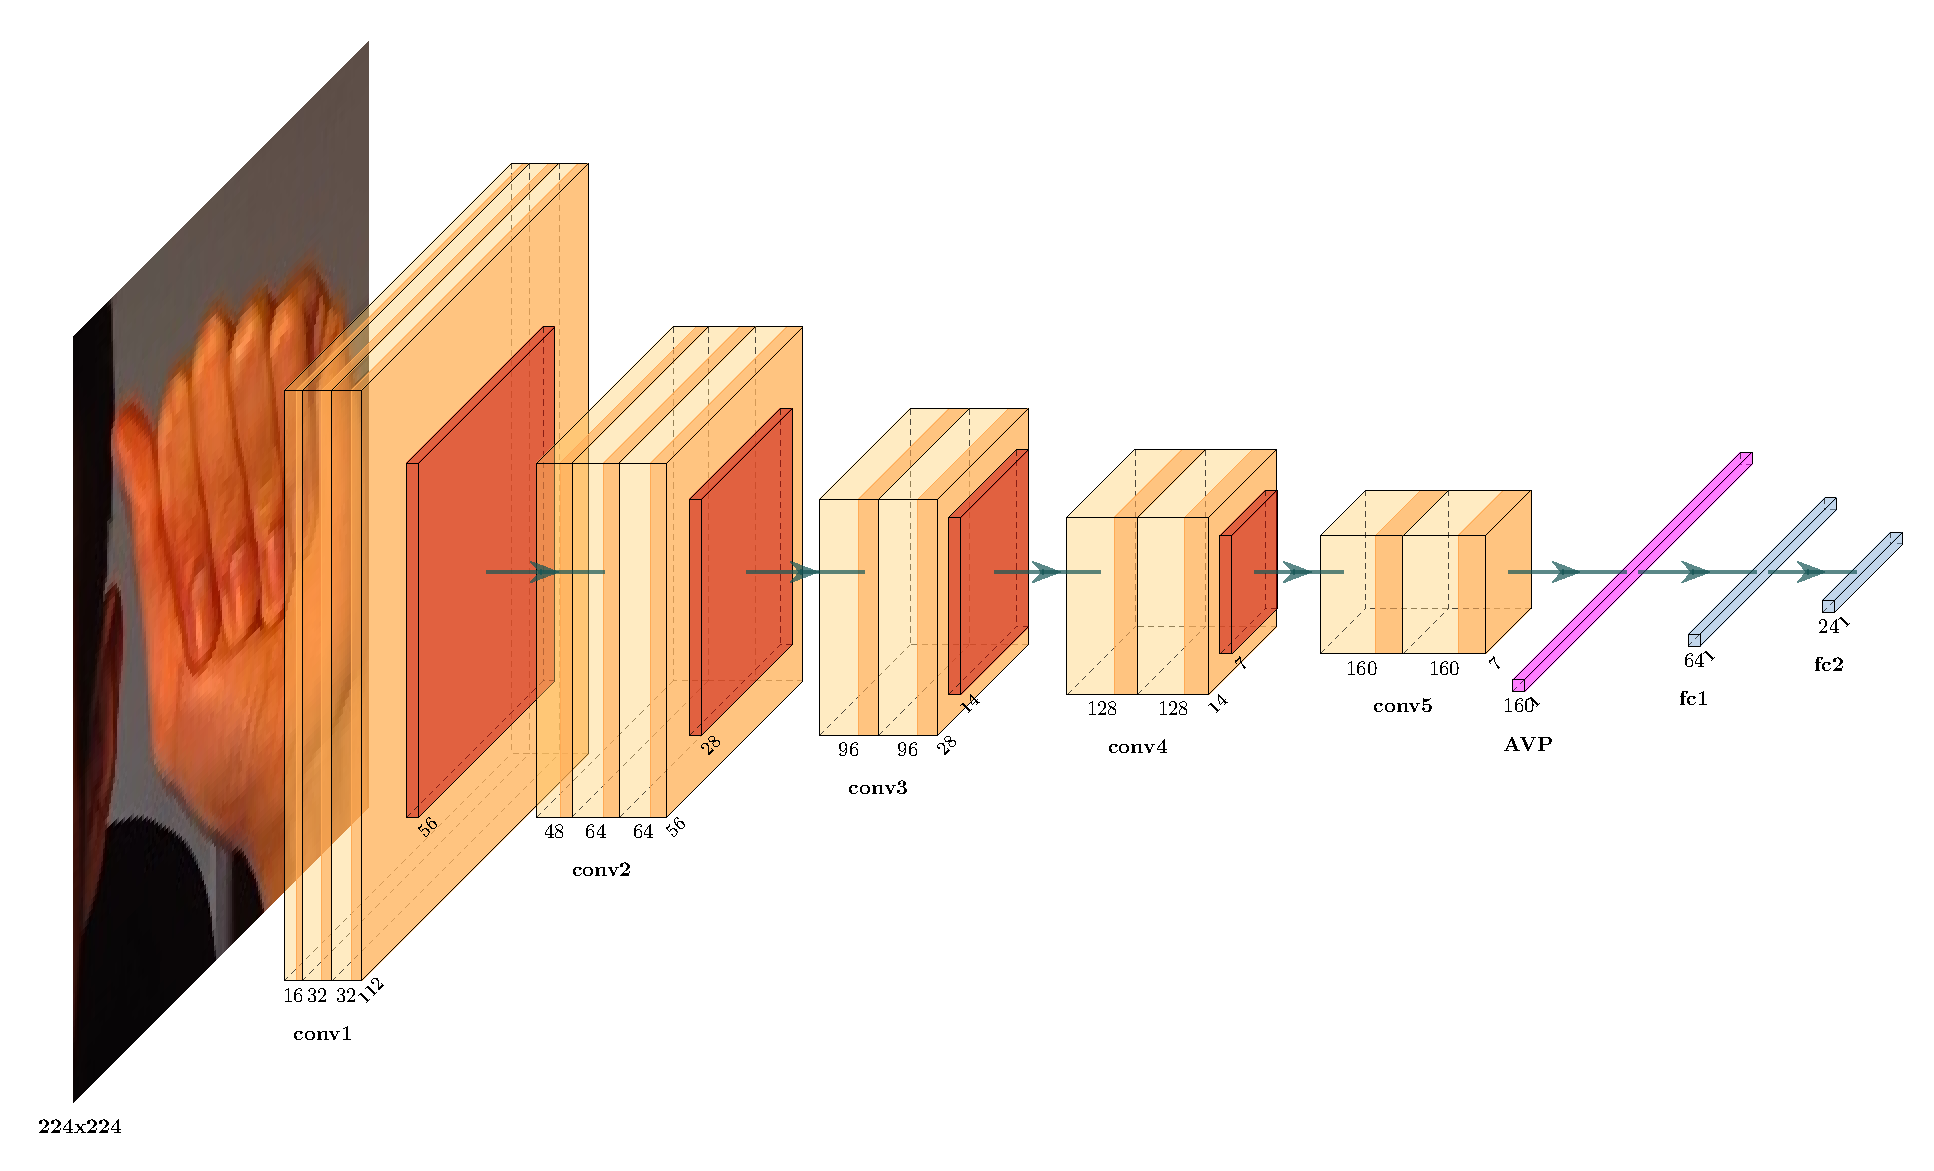
\includegraphics[width=\textwidth]{images/2-recunoasterea-asl/VladimirNetArchitecture.pdf}
  \caption[Arhitectura VladimirNet]{\textbf{Arhitectura VladimirNet}. \textit{Ilustrăm arhitectura modelului utilizat în lucrare, denumită \textbf{VladimirNet}. Conține un număr total de 927.496 de parametri. Prima imagine din stânga reprezintă imaginea care este transmisă modelului, cu dimensiunea inițială de 224 \times 224. Blocurile convoluționale sunt notate cu conv1, conv2, conv3 conv4, conv5. Fiecare strat este evidențiat cu galben transparent și are notat dedesubt numărul de canale în urma aplicării operației de convoluție. Straturile de batch normalization și ReLU sunt ilustrate cu portocaliu, iar culoarea roșie indică operația de max pooling. AVP reprezintă operația de adaptive average pooling. Fc1 și fc2 sunt straturile dense ale clasificatorului. Diagrama a fost construită cu ajutorul bibliotecii \LaTeX, \textbf{PlotNeuralNet}} \cite{haris_iqbal_2018_2526396}.}
  \label{fig:diagrama_vladimirnet}
\end{figure}

\begin{enumerate}
    \item Primul bloc este format din trei straturi convoluționale. Primul strat extinde numărul canalelor de la trei (RGB) la 16, crescând adâncimea și micșorând imaginea la $112 \times 112$, utilizând kernel de $5 \times 5$ și $stride = 2$ cu $padding = 2$. Dimensiunea este redusă la $112 \times 112$ pentru a nu consuma prea multă memorie la început, având în vedere dimensiunea kernel-ului de $5 \times 5$ care poate fi mai costisitor din punct de vedere computațional. Al doilea strat din blocul curent extinde din nou numărul de canale la 32 și utilizează tot un kernel de $5\times 5$, concentrându-se în continuare pe caracteristici generale. Ultimul strat, la fel ca toate straturile din finalul blocurilor convoluționale ale arhitecturii, nu adâncește imaginea, ci păstrează numărul de canale din stratul anterior, însă de data aceasta folosind un kernel de $3 \times 3$. Scopul ultimului strat este rafinarea și consolidarea trăsăturilor învățate pâna atunci, înainte de stratul de max pooling, cu rolul de a reduce dimensiunea spațială la jumătate. Fiecare bloc convoluțional din cele descrise în continuare este urmat de un strat de max pooling, cu excepția ultimului. 
    \item Al doilea bloc funcționează pe același principiu: 3 straturi convoluționale, ultimul păstrând numărul de canale, însă de acum înainte toate straturile utilizează un kernel cu dimensiunea de $3 \times 3$.
    \item Al treilea, al patrulea și al cincilea bloc conțin numai 2 straturi convoluționale, pentru a controla complexitatea modelului, având în vedere că ultimul strat atinge un număr de 160 de canale.
    \item Ultimul bloc convoluțional nu mai este urmat de max pooling, ci de adaptive average pooling, strat care reduce dimensiunea spațială a fiecărei hărți la $1 \times 1$, rezultând un vector cu $160$ de valori.
    \item În final, vectorul rezultat este transmis către clasificatorul format din două straturi complet conectate. Primul strat este urmat de ReLU și un strat de \textit{dropout} cu $p=0.45$, care dezactivează aleatoriu $45\%$ dintre neuroni și conexiunile acestora, metodă necesară pentru a combate overfitting-ul \cite{dropout1, dropout2}. Ultimul strat dens este cel care ne oferă predicția.
\end{enumerate}
 
De asemenea, este important să menționăm că ponderile sunt inițializate prin metoda \textit{Kaiming}, care folosește valori dintr-o distribuție normală. Scopul acestei inițializări este de a evita gradienți care tind spre 0 (\textit{vanishing gradient)} sau care „explodează” (\textit{exploding gradient)} 
\cite{kaiming_w_init}.

\section{Antrenarea modelului}
Antrenarea modelului a fost realizată în platforma \textbf{Google Colab} \cite{colab}, folosind un \textit{GPU} \textbf{NVIDIA L4}.

\textbf{Funcția de pierdere}. Pentru evaluarea predicțiilor oferite de către model, este utilizată entropia încrucișată (în engl. \textit{Cross Entropy}) implementată cu ajutorul clasei \textit{CrossEntropyLoss} din PyTorch, după formula:

\begin{equation}
    L = - \sum_{i=1}^{C}y_i \cdot \log(\hat{y}_i)
\end{equation}
unde $C$ este numărul de clase posibile, $y_i$ reprezintă vectorul \textit{one-hot} a etichetei corecte, iar $\hat{y}_i$ este vectorul rezultat din ultimul strat dens, asupra căruia este aplicată funcția de activare \textit{softmax}.

Ca metodă de regularizare, vom folosi și o tehnică denumită \textit{label smoothing} (netezirea etichetelor) \cite{label_smooth}, astfel încât $y_i$, vectorul one-hot \textit{hard} utilizat de funcția cross entropy, este înlocuit cu unul soft care îndepărtează modelul de predicții excesiv de încrezătoare.


\textbf{Algoritmul de optimizare}. Pentru antrenarea modelului, s-a hotărât utilizarea algoritmului de optimizare \textit{AdamW} \cite{adamw_article}, bazat pe Adam (Adaptive Moment Estimation) \cite{adam_article}. Îmbunătățirea adusă de către AdamW algoritmului de optimizare Adam constă în decuplarea 
penalizării ponderilor mari (în engl. \textit{weight decay}) de calculul gradientului, astfel încât formula pentru actualizarea ponderilor este următoarea: 

\begin{equation}
    \theta_{t+1} = \theta_t - \eta \cdot \left(\frac{\hat{m}_t}{\sqrt{\hat{v}_t} + \epsilon} + \lambda \cdot \theta_t\right)
\end{equation}
unde $\theta_{t}$ sunt ponderile în pasul $t$, $\eta$ este rata de învățare, $\hat{m}_t$ este media exponențială a gradientelor în pasul $t$, $\hat{v}_t$ este  media exponențială a pătratelor gradientelor în pasul $t$, iar $\lambda$ reprezintă factorul de penalizare a greutăților.


\textbf{Hiperparametri}. Pentru optimizator, am ales o rată de învățare $\eta = 1\times 10^{-3}$, aceasta fiind valoarea implicită din clasa \textit{AdamW} a bibliotecii PyTorch. Pe parcursul învățării, $\eta$ este ajustat treptat, la final având o valoare de $1\times10^{-5}$. Ajustarea este facilitată de clasa \textit{CosineAnnealingLR} din PyTorch, care actualizează $\eta$ la finalul fiecărui batch. Scopul acestei ajustări este de a scoate modelul din anumite minime locale nedorite, iar pe parcursul învățarii, actualizările parametrilor să fie din ce în ce mai fine.

După cum am menționat mai devreme, etichetele sunt „netezite” înainte de a fi oferite funcției de pieredere, cu un factor de netezire $\epsilon = 0.15$, penalizând predicțiile excesiv de încrezătoare.

Timpul de antrenament este de 60 de epoci, cu mărimea batch-ului de 64 de exemple.

Pentru weight decay, utilizăm o valoare de $1 \times 10^{-6}$. Valoarea implicită pentru weight decay este de $1\times10^{-2}$, însă o valoare așa ridicată conduce către o învățare mai lentă.

\section{Evaluarea modelului}

În timpul antrenării, la finalul fiecărei epoci, performanța modelului era evaluată pe setul de validare. Modelul a fost salvat în fiecare punct maxim al acurateții obținute pe setul de validare.

Evaluările au fost create și vizualizate cu ajutorul bibliotecilor \textbf{scikit-learn} \cite{scikit-learn}, \textbf{Matplotlib} \cite{matplotlib} și \textbf{seaborn} \cite{seaborn}.

Putem observa în Figura~\ref{fig:train_val_acc}
evoluția modelului pe parcursul celor 60 de epoci. Acuratețea maximă pe setul de antrenare este de $92,45\%$, iar pe setul de validare de $92,27\%$. Datorită augmentărilor puternice și dificultății setului de antrenare, comparativ cu cel de validare, acuratețea setului de validare s-a menținut aproape constant deasupra acurateții setului de antrenare, iar spre final, acuratețea setului de antrenare ajungând să stagneze, cu o ușoară tendință descendentă. 

În Figura~\ref{fig:train_val_loss} putem observa cum funcția de pierdere scade treptat, indicând o învățare continuă.


\begin{figure}[H]
  \centering
  \begin{subfigure}{0.49\textwidth}
    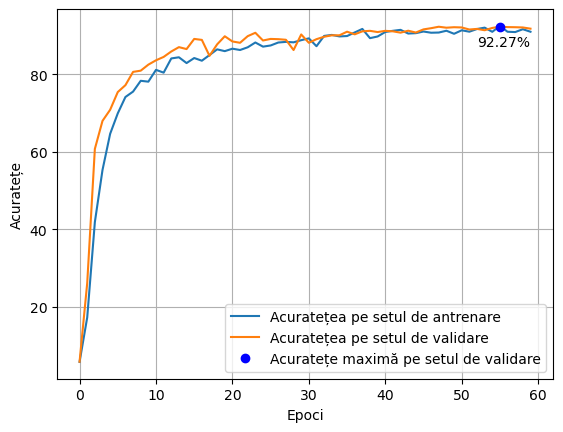
\includegraphics[width=\linewidth]{images/2-recunoasterea-asl/train_val_accs.png}
    \caption{}
    \label{fig:train_val_acc}
  \end{subfigure}
  \begin{subfigure}{0.49\textwidth}
    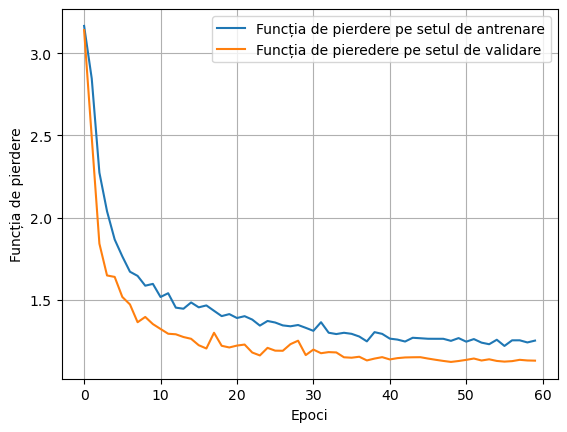
\includegraphics[width=\linewidth]{images/2-recunoasterea-asl/train_val_loss.png}
    \caption{}
    \label{fig:train_val_loss}
  \end{subfigure}
  \caption[Vizualizarea antrenării]{\textbf{Vizualizarea antrenării}. \textit{(a) ilustrează evoluția acurateții pe parcursul celor 60 de epoci de antrenare; (b) ilustrează evoluția funcției de pierdere pe parcursul antrenării.}}
  \label{fig:train_val_acc_loss}
\end{figure}



După obținerea unor rezultate satisfăcătoare asupra testului de validare, modelul a fost evaluat și prin prisma setului de testare, obținând o acuratețe de $91,05\%$. În Figura~\ref{fig:conf_matrix_test_set} poate fi analizată matricea de confuzie obținută în urma evaluării rezultatelor setului de testare. Literele G și H sunt asemănătoare, la fel și literele N și M, motiv pentru care modelul le confundă mai des. Litera X este de asemenea confundată cu litera C, iar litera Y cu litera A.

\begin{figure}[H]
  \centering
  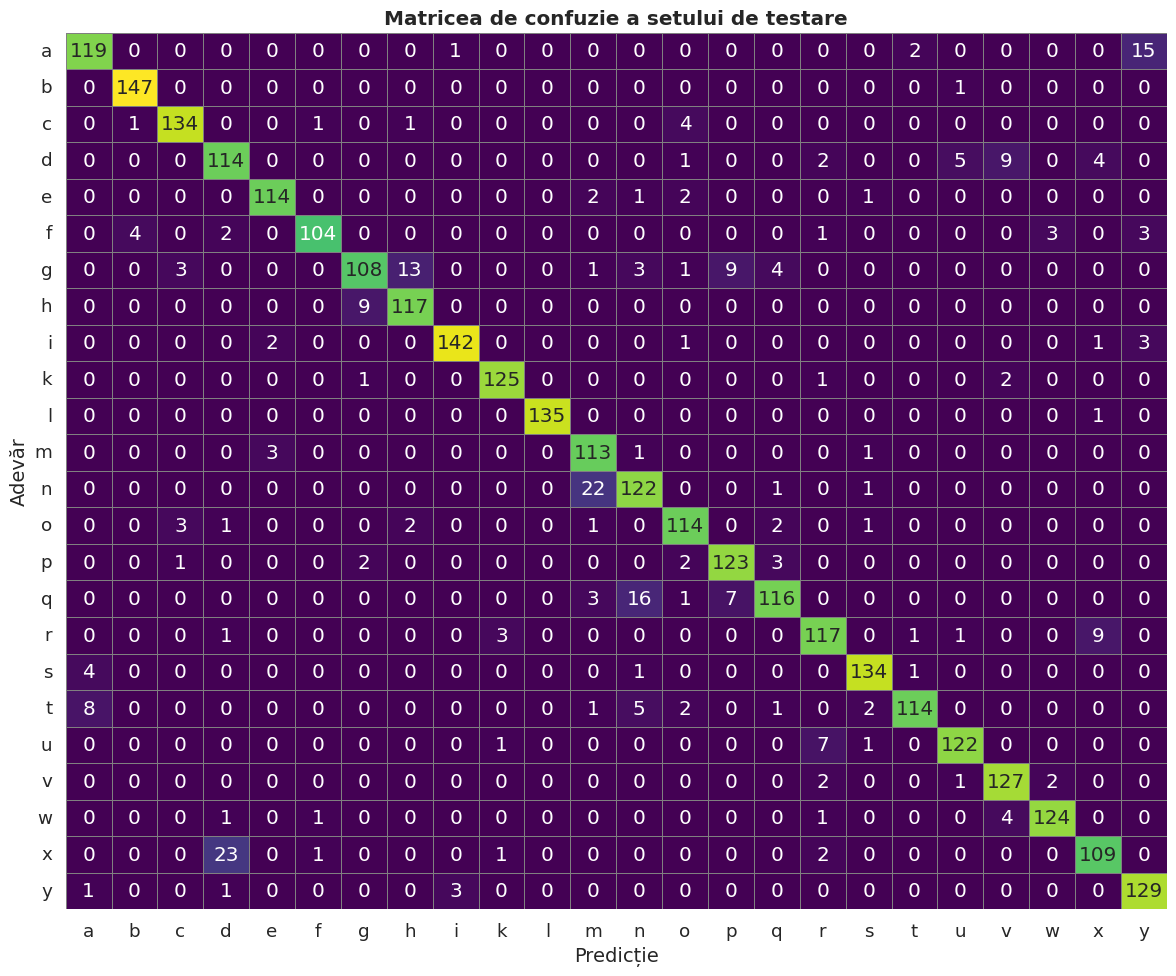
\includegraphics[width=0.55\textwidth]{images/2-recunoasterea-asl/conf_matrix_test_set.png}
  \caption[Matricea de confuzie a setului de testare]{\textbf{Matricea de confuzie a setului de testare}. \textit{Ilustrăm matricea de confuzie cu ajutorul unei hărți termice. Diagonala principală reprezintă numărul de exemple prezise corect pentru fiecare literă.}}
  \label{fig:conf_matrix_test_set}
\end{figure}

Mai departe, în Figura~\ref{fig:acc_per_class} poate fi analizată acuratețea pentru fiecare literă. Literele cele mai ușor de recunoscut de către modelul creat sunt B și L, cu acuratețe de $99,3\%$, iar cele care ridică probleme sunt G, cu o acuratețe de $76,1\%$, și X, cu acuratețe de $80,1\%$.

\begin{figure}[H]
  \centering
  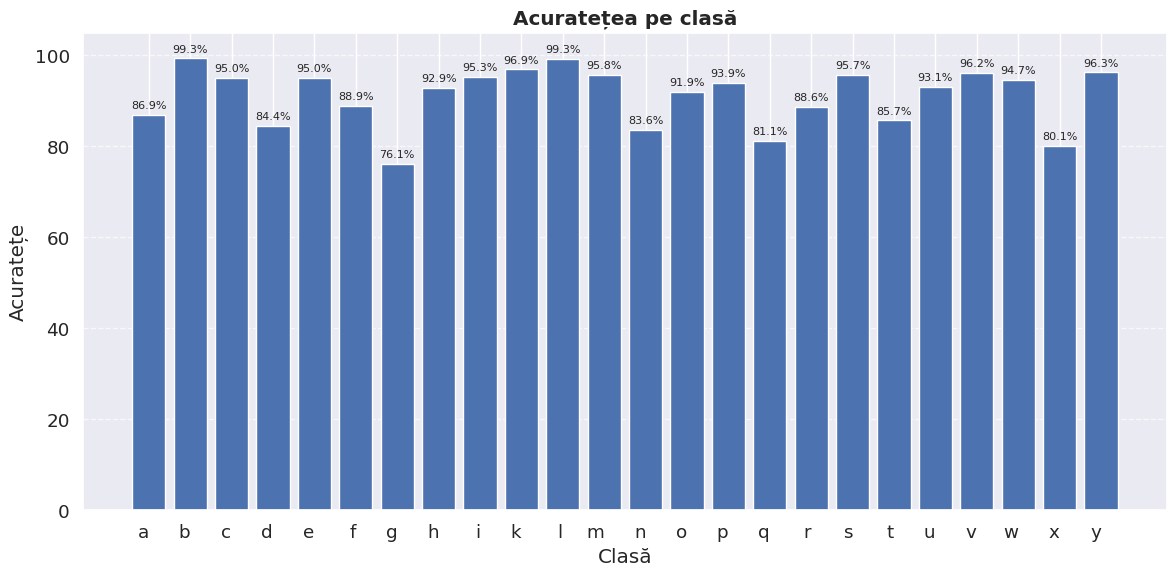
\includegraphics[width=0.7\textwidth]{images/2-recunoasterea-asl/acc_per_class.png}
  \caption[Acuratețea pe clasă]{\textbf{Acuratețea pe clasă}. \textit{Ilustrăm acuratețea predicțiilor pentru fiecare literă. Acuratețea este notată în vârful dreptunghiurilor reprezentative pentru clasa respectivă.}}
  \label{fig:acc_per_class}
\end{figure}

În final, am creat un raport de clasificare. În Tabela~\ref{tab:classif_report} putem observa cum litera G are un scor \textit{recall} scăzut (0.76), ceea ce înseamnă că există dificultăți în a recunoaște acea clasă. Combinând acest fapt cu datele din matricea de confuzie, putem concluziona că de multe ori, modelul are tendința să confunde G cu H, clasificând litera G ca fiind H. Mai mult de atât, chiar dacă litera Y are o acuratețe ridicată, poate fi observat cum scorul \textit{precision} este mai scăzut (0.86), sugerând faptul că modelul tinde să prezică Y și în situații în care aceasta nu este litera corectă.

\begin{table}[H]
\centering
\scriptsize
\begin{tabular}{c c c c c}
\toprule
\textbf{Clasă} & \textbf{Precizie} & \textbf{Recall} & \textbf{Scor F1} & \textbf{Număr exemple} \\
\midrule
a & 0.90 & 0.87 & 0.88 & 137 \\
b & 0.97 & 0.99 & 0.98 & 148 \\
c & 0.95 & 0.95 & 0.95 & 141 \\
d & 0.80 & 0.84 & 0.82 & 135 \\
e & 0.96 & 0.95 & 0.95 & 120 \\
f & 0.97 & 0.89 & 0.93 & 117 \\
g & 0.90 & 0.76 & 0.82 & 142 \\
h & 0.88 & 0.93 & 0.90 & 126 \\
i & 0.97 & 0.95 & 0.96 & 149 \\
k & 0.96 & 0.97 & 0.97 & 129 \\
l & 1.00 & 0.99 & 1.00 & 136 \\
m & 0.79 & 0.96 & 0.87 & 118 \\
n & 0.82 & 0.84 & 0.83 & 146 \\
o & 0.89 & 0.92 & 0.90 & 124 \\
p & 0.88 & 0.94 & 0.91 & 131 \\
q & 0.91 & 0.81 & 0.86 & 143 \\
r & 0.88 & 0.89 & 0.88 & 132 \\
s & 0.95 & 0.96 & 0.95 & 140 \\
t & 0.97 & 0.86 & 0.91 & 133 \\
u & 0.94 & 0.93 & 0.93 & 131 \\
v & 0.89 & 0.96 & 0.93 & 132 \\
w & 0.96 & 0.95 & 0.95 & 131 \\
x & 0.88 & 0.80 & 0.84 & 136 \\
y & 0.86 & 0.96 & 0.91 & 134 \\
\bottomrule
\end{tabular}
\caption[Raport de clasificare]{Pentru fiecare clasă, raportăm numărul de exemple testate și scorurile: precizie, recall și F1.}
\label{tab:classif_report}
\end{table}


\section{Evaluare experimentală}

Înainte de a avea arhitectura finală a rețelei neuronale convoluționale, au fost încercate diferite modele și tipuri de imagini.

În faza incipientă, imaginile au fost utilizate în forma lor originală, fără decuparea mâinii cu ajutorul MediaPipe Hands. Pentru a ne asigura că setul de date este corect, am antrenat un model cu arhitectura ResNet50 timp de 50 de epoci, obținând o acuratețe de $89.5\%$ pe setul de validare. După ce am confirmat corectitudinea setului de date, s-a optat pentru arhitecturi mai simple, deoarece ResNet50 are aproximativ 25M parametri, ceea ce este considerat ineficient pentru rularea locală pe dispozitive mobile.

Încercând cu arhitecturi proprii, am ajuns la acuratețe de aproximativ $68\%$, cu modele care au între 300.000 și 10.000.000 de parametri. Principalele dificultăți întâmpinate au fost reprezentate de subînvățare și supraînvățare. Pe lângă numărul de parametri, arhitectura a ridicat probleme și în funcție de așezarea straturilor convoluționale și rata creșterii numărului de canale. În cazul în care dublam numărul canalelor la fiecare strat convoluțional, de exemplu 3 \rightarrow\space 32 \rightarrow\space 64 \rightarrow\space 128 \rightarrow\space 256 \rightarrow\space 512, modelul devenea rapid prea complex și evaluarea începea să indice memorarea setului de date.

Printre algoritmii de ajustare a ratei de învățare, se numără \textit{ReduceLROnPlateau}, care reduce $\eta$ când învățarea stagnează, și \textit{CosineAnnealingWarmRestarts}, care resetează $\eta$ la un anumit punct, readucând rata de învățare la valoarea inițială, pentru a scăpa din minime locale și a încerca alte „drumuri” către convergență. În ambele cazuri, rezultatele nu erau cele așteptate, cele mai bune rezultate fiind observate prin utilizarea algoritmului CosineAnnealing.

Un punct de cotitură în cadrul testelor noastre a fost atins când am hotărât să utilizăm MediaPipe Hands pentru a extrage cadre cu mâinile. Acuratețea a început să crească considerabil, atingând deseori $90\%$, cu arhitecturi care conțineau aproximativ 1.000.000 de parametri. 

Pe lângă modelul prezentat în Capitolul~\ref{cap:cap2}, am antrenat și un MobileNetV3Large \cite{mobilenetv3}, care a atins acuratețe de $95,96\%$ pe setul de validare. Scopul acestui model era de a-l introduce ca opțiune de utilizare în aplicație pentru dispozitive performante, însă după convertirea într-un format compatibil cu Android, timpul de detecție pe cadru creștea considerabil și nu am putut identifica cauza precisă.

În ceea ce privește augmentarea datelor, trebuie menționat că, în cazul CutMix și Mixup, etichetele trebuie reprezentate ca vectori soft, conform articolului original dedicat metodei CutMix. Autorii menționează că utilizarea doar a etichetei dominante oferă rezultate mai bune decât absența aceastei metode de augmentare, însă rezultatele cele mai bune vor fi obținute prin utilizarea etichetelor soft. În urma experimentelor noastre, am observat că prin utilizarea etichetelor soft, a arhitecturii dezvoltate și a hiperparametrilor prezentați în această lucrare, acuratețea maximă obținută a fost de doar $89,15\%$.